\newpage
\section{Math101 opgaver til 3. gang}
\begin{enumerate}
	
	\item Lad $f(x)=3x^2+2x+1$. Bestem $f(-1)$ og $f(2)$.
	
	\item \label{it:5} Cirklen med ligning $x^{2} +(y-1)^{2}=1$ er tegnet i Figur~\ref{fig:5}.
	\begin{itemize}
		\item Findes en funktion $f\colon [-1,1]\to [0,2]$ så grafen for $f$ svarer til cirklen i Figur~\ref{fig:5}?
		\item Bestem en funktion $f_+\colon [-1,1]\to [1,2]$ så grafen for $f_+$ svarer til den øvre halvcirkel i Figur~\ref{fig:5}. (Hint: isoler $y$ i cirklens ligning.)
		\item Bestem en funktion $f_-\colon [-1,1]\to [0,1]$ så grafen for $f_-$ svarer til den nedre halvcirkel i Figur~\ref{fig:5}.
	\end{itemize}	
	\begin{figure}
		\centering
		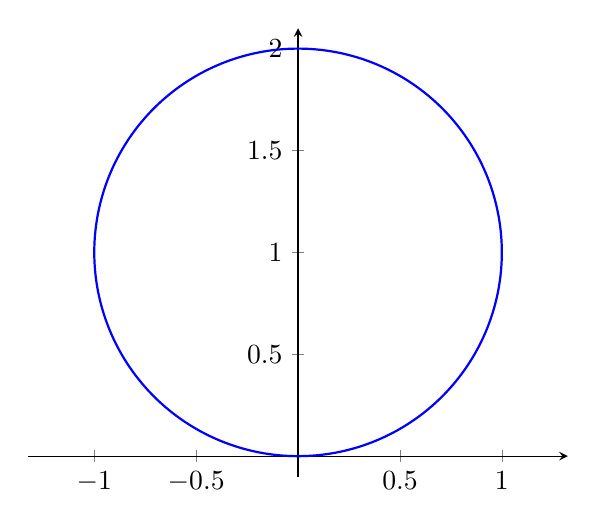
\begin{tikzpicture}
		\begin{axis}[xmin=-1.1,xmax=1.1,ymin=-0.1,ymax=2.1,axis x line=center,
		axis y line=center,axis equal, restrict y to domain=-2:2]
		\addplot[thick,blue,domain=0:2*pi,samples =800] ({cos(deg(x))},{1+sin(deg(x))});
		\end{axis}
		\end{tikzpicture}
		\caption{Opgave~\ref{it:5}.}
		\label{fig:5}
	\end{figure}

	
	\item Lad $f(x)=3x-2$ og $g(x)=\frac{1}{3}x+\frac{2}{3}$. Bestem forskriften for $f\circ g$.

	\item Bestem den størst mulige definitionsmængde for funktionerne:
	\begin{align*}
	f(x)=\frac{1}{1-x},&& g(x)=\frac{1}{1-x^2},&& h(x)=\sqrt{2x-3}.
	\end{align*}
	
	
	\item  Lad $f,g$ være givet ved $f(x)=\sqrt{x}$ og $g(x)=1/(1+x)$ på domænet $(0,\infty)$. Udregn $(f\circ g)(1)$ og $(g\circ f)(1)$. Er $f\circ g=g\circ f$?
	
	\item Bestem skæringspunktet mellem $f(x)=3x+1$ og $g(x)=-x+2$.	
	
		\item Lad $f(x)=1$ og $g(x)=2x+3$. Bestem $f\circ g$ og $g\circ f$.
	
		
	\item Bestem den størst mulige definitionsmængde for funktionerne
	\begin{align*}
	f(x)=\frac{1}{(1+x^2)^\frac{1}{2}},&& g(x)=\frac{2}{x^2-4x+3},&& h(x)=\sqrt{-x^2+2x}.
	\end{align*}
	


	\item Bestem funktioner $f$ og $g$ så $(f\circ g)(x)=e^{2x^2-1}$.
	
	\item Bestem alle skæringspunkter mellem $f(x)=x^2+4x+4$ og $g(x)=2x+3$.
	
	\item Bestem funktioner $f$, $g$ og $h$ så at $(f\circ g\circ h)(x)=\sin^2(3x)$. (Hint: $ \sin^2(x)=(\sin(x))^2 $.)
	
	\item Lad $f(x)=3(\frac{1}{x-2})^2$, $g(x)=\frac{1}{x}$ og $h(x)=\sqrt{x}+2$ være funktioner på domænet $]2,\infty[$. Bestem
	\begin{align*}
	f(g(x)),&& f(h(x)),&& h(g(x)),&& h(f(x)),&&g(f(h(x))).
	\end{align*} 
	
		\item\label{it:fun3} Er kurven i Figur~\ref{fig:fun3} grafen for en funktion?
	\begin{figure}
		\centering
		\begin{tikzpicture}
		\begin{axis}[xmin=-5,xmax=5,ymin=-5,ymax=5,axis x line=center,
		axis y line=center, restrict y to domain =-5:5]
		\addplot[data cs=polar, thick,blue,samples=200, domain= 0:180] ({x}, {3*sin(x)*cos(x)/(sin(x)^3+cos(x)^3)});
		\end{axis}
		\end{tikzpicture}
		\caption{Opgave~\ref{it:fun3}.}
		\label{fig:fun3}
	\end{figure}
	
	
		
	\item Skitser grafen for en funktion som opfylder alle nedenstående puntker:
	\begin{enumerate}
		\item har domæne $[-1,1]$,
		\item går gennem punkterne $(-1,0)$ og $(1,1)$,
		\item skærer $y$-aksen i $-1$,
	\end{enumerate}
	
\end{enumerate}